\section{Working hours}

\subsection{Sleep rythm}
To evaluate the significance of the punchcard in terms of sleep rhythm analysis, a small survey in a closed community has been made.
A selected group of ten people, who know each other well has been selected, for this purpose.
Furthermore a subset of four people has been chosen, which were going to be evaluated.
All ten people then needed to assign the punchcard of the chosen subset to a specific person.

\begin{figure}[H]
    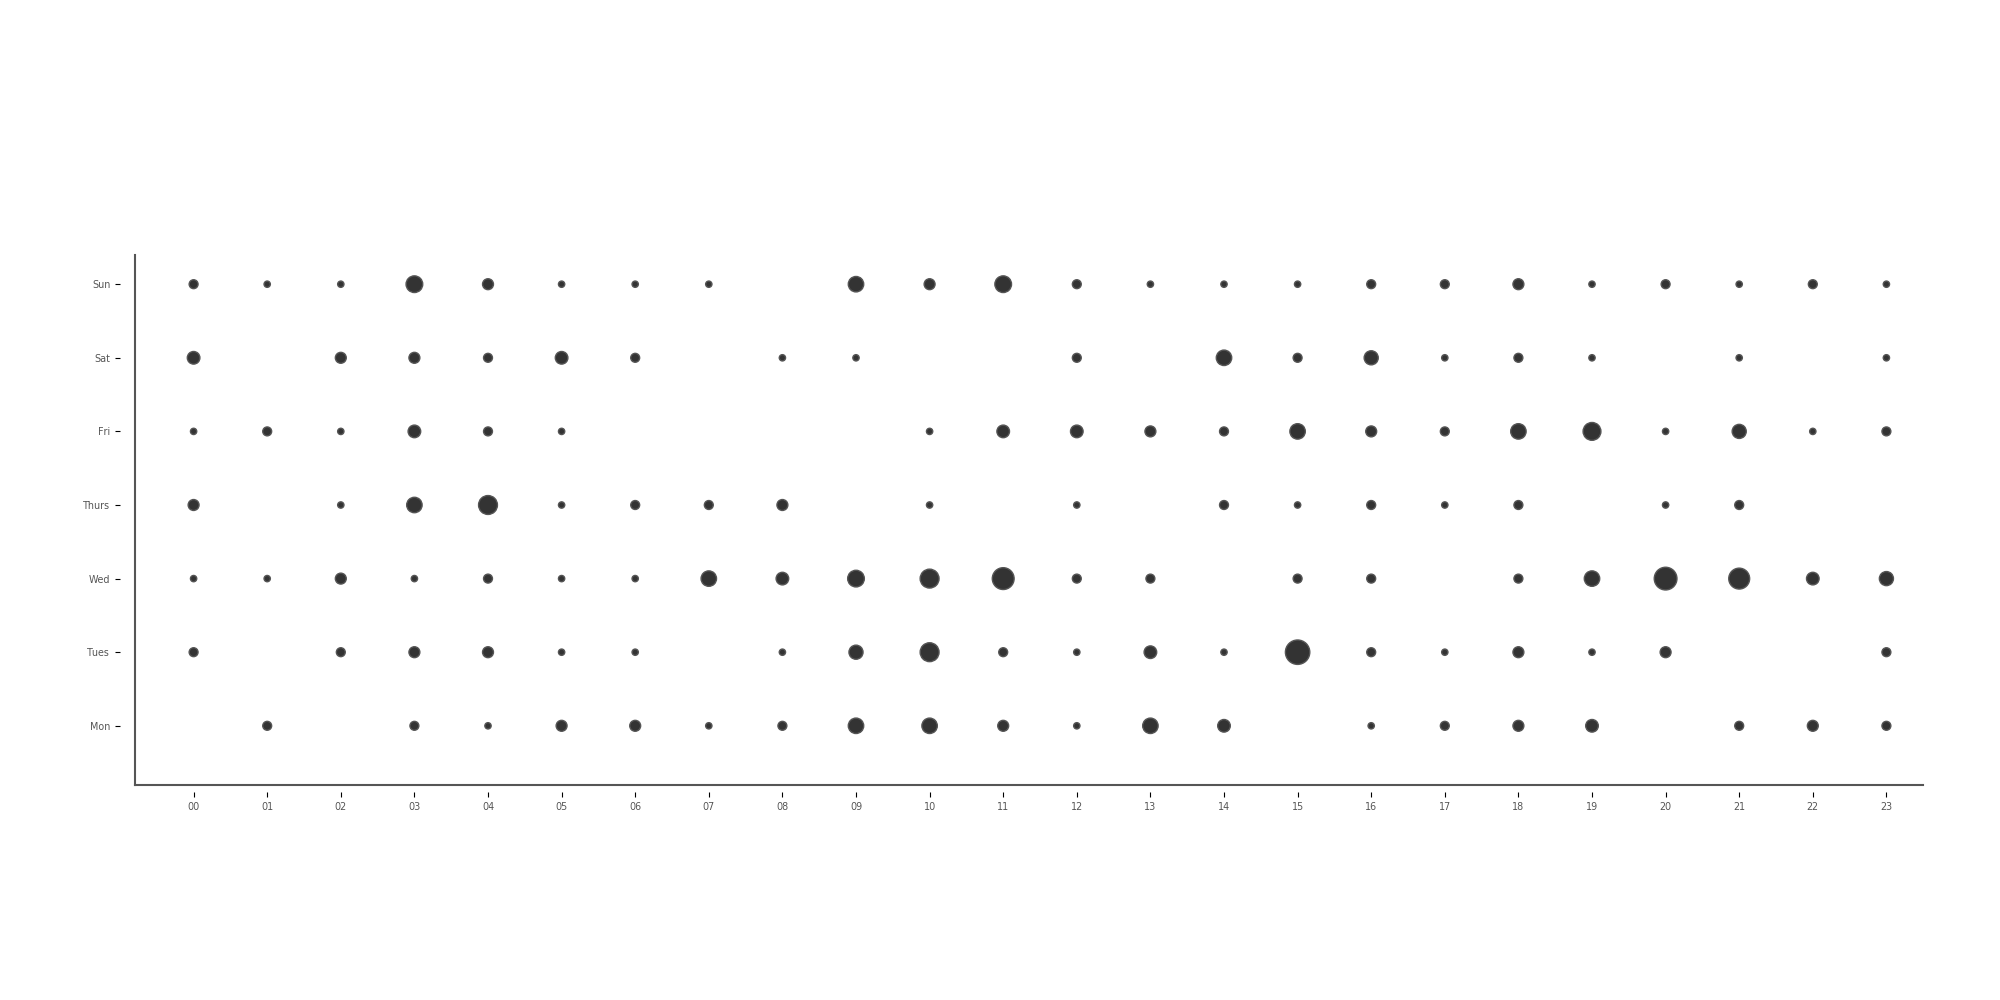
\includegraphics[scale=0.32]{./graphs/analysis/random-punchcard}
    \centering
    \caption{Punchcard of an user without an irregular sleep rhythm.}\label{fig:random-sleep-rhythm}
\end{figure}

\subsection{Employee or Open-Source Contributor}
To determine whether a punchcard could be used to distinguish between an employee or an open-source contributor, the results of the clustering described in Section~\ref{punchcard-implementation} has been utilized.
For this approach two assumptions have been made.
An usual employee works between Monday and Friday and only as an exception during the weekend.
An open-source developer works outside of the usual work shifts, which means early and late during weekdays and at the weekend.

For each assumption two representative clusters have been chosen and ten random persons have been selected for each cluster.
The manual verification is conducted by checking if the contributor mainly contributes to repositories which belong to the registered employee.
In case no employee exists, it is examined whether the contributor pushes to their own or open-source projects or rather to the repositories of a specific company.

\begin{figure}[H]
    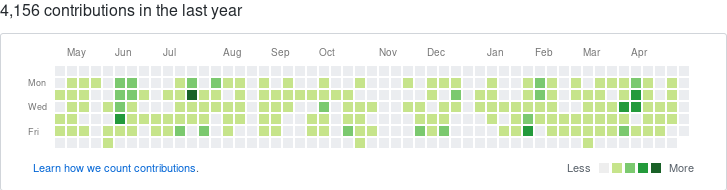
\includegraphics[scale=0.6]{./graphs/contribution-overview-alxhub}
    \centering
    \caption{Github contribution overview a Google developer with the Github nickname alxhub.}\label{fig:random-sleep-rhythm}
\end{figure}

It provides a good overview of the usual weekday work pattern over the last year and allows to quickly inspect the repositories a contributor committed to at a specific date.

\begin{figure}[H]
    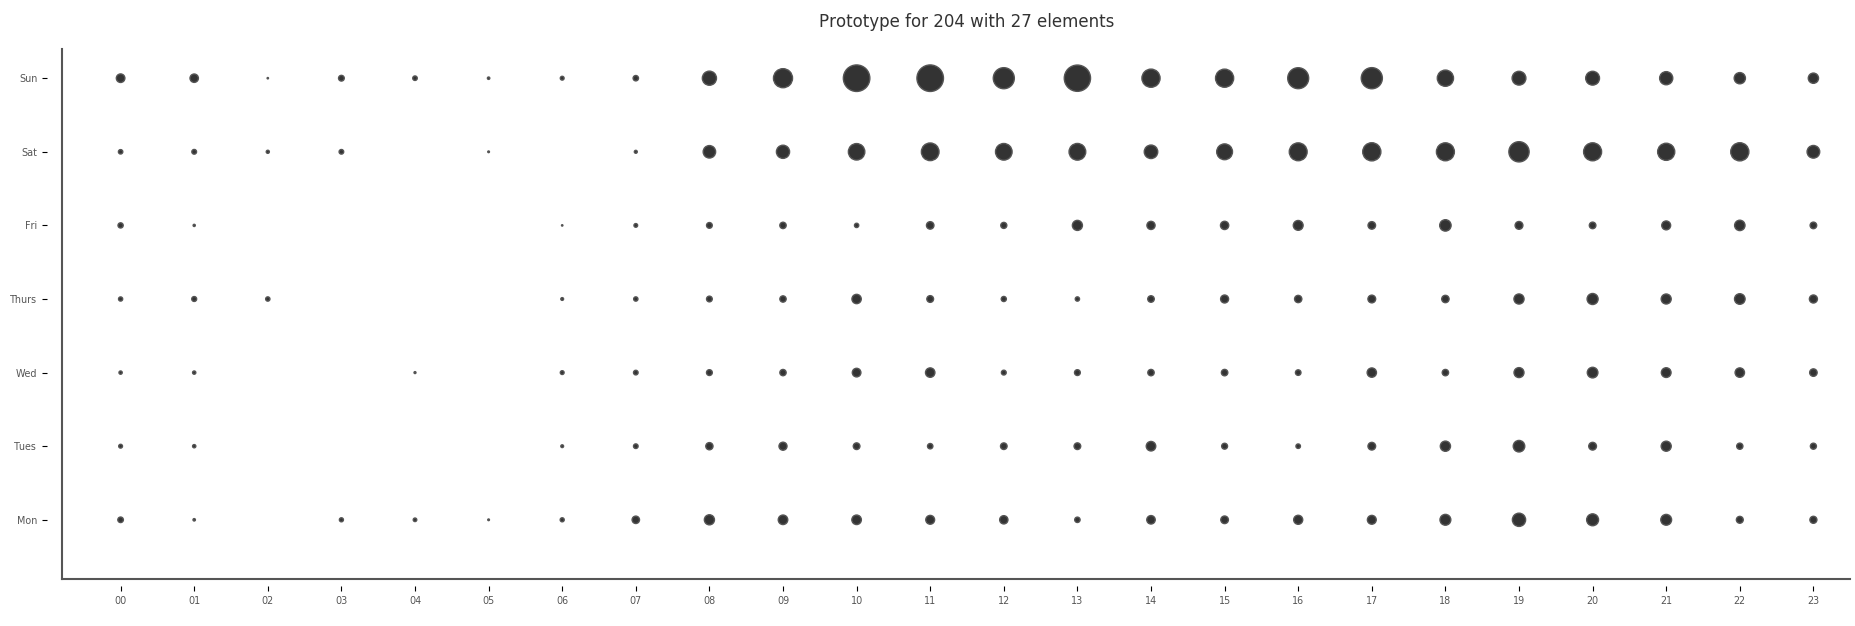
\includegraphics[scale=0.32]{./graphs/analysis-affinity/204}
    \centering
    \caption{Punchcard of an example from an affinity propagation cluster with a weekend tendency.}\label{fig:random-sleep-rhythm}
\end{figure}

The representatives for the usual five-day week work behaviour were surprisingly prices.
About 97\% of considered contributors were mainly working on projects of their companies, with sometimes occasional commits to their open source projects.

\begin{figure}[H]
    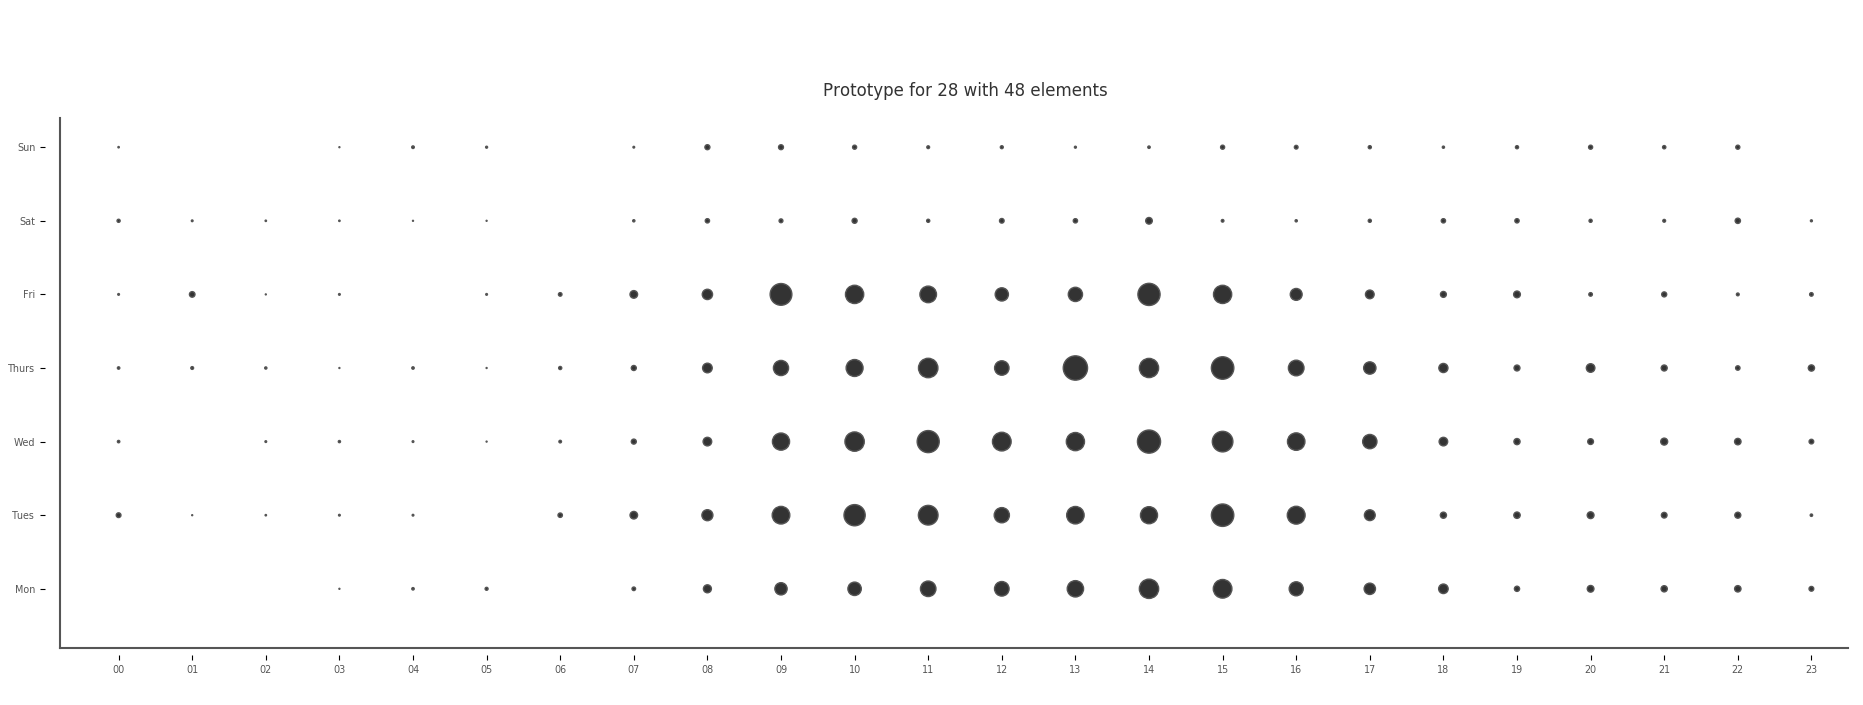
\includegraphics[scale=0.32]{./graphs/analysis-affinity/28}
    \centering
    \caption{Punchcard of an example of an affinity propagation cluster with normal work shifts.}\label{fig:random-sleep-rhythm}
\end{figure}
